\documentclass[a4paper,12pt]{article} 

\usepackage[a4paper, top=3cm, bottom=3cm, left=2cm, right=2cm]{geometry}
\usepackage{amsmath,amsthm,amssymb}
\usepackage{cmap}					% поиск в PDF
\usepackage[utf8]{inputenc}			% кодировка исходного текста
\usepackage[english]{babel}     	% локализация и переносы
\usepackage{csquotes}
\usepackage{multicol}
\usepackage{tikz}
\usetikzlibrary{positioning}

\bibliographystyle{abbrv}

\usepackage[ruled,linesnumbered]{algorithm2e}

\newtheorem{claim}{Claim}

\newcommand{\cq}[1]{\ensuremath{\mathsf{CQ}_{#1}}}
\newcommand{\query}[3]{\ensuremath{{#1}({#2})\:{:}{-}\:{#3}}}
\newcommand{\rr}{\mathsf{RR}}
\newcommand{\ranf}{\mathsf{RANF}}
\newcommand{\srnf}{\mathsf{SRNF}}
\renewcommand{\phi}{\varphi}

\begin{document}

\begin{center}
{\LARGE\bfseries Foundations of Databases}\\[3mm]

{\Large Coursework 2}\\[5mm]

Lorenz Leutgeb\\\texttt{lorenz.leutgeb@stud-inf.unibz.it}\\[2mm]
Anastassiya Pustozerova\\\texttt{anastassiya.pustozerova@stud-inf.unibz.it}
\end{center}

\section{Safety of Positive Queries}

\begin{claim}
The safety of simple positive queries is decidable.
\end{claim}

\begin{proof}[Sketch of Proof] We specify an algorithm. Similar to the approach presented in the lecture we first translate $\phi$ into a normal form to allow for a concise rule-based formulation.

We choose (a subset of) SRNF as our normal form, and re-use the algorithm given in \cite[Section 5.4, p.\ 83]{alice} to translate a simple positive formula to SRNF. We call it $\srnf$. Note that some rules of this algorithm will never be applicable to simple positive formulae: universal quantification, implication and negation are not included in the definition of simple positive formulae. This hints why we only need to consider a subset of SRNF, intuitively \emph{simple positive SRNF}. Also note that the rewrite rules preserve equivalence and therefore $\phi$ is safe if and only-if $\srnf(\phi)$ is safe.

From here, we can use $\srnf$ and the algorithm below (adapted from \cite[Algorithm 5.4.3, p.\ 84]{alice} to decide safety of formulae in simple positive SRNF) to decide safety of simple positive formulae: A simple positive formula $\phi$ is safe if and only-if $\rr(\srnf(\phi))$ returns the set of all free variables of $\phi$.

\begin{algorithm}
  \KwIn{A formula $\phi$ in simple positive SRNF.}
  \KwOut{The subset of free variables of $\phi$ that are range-restricted, or $\bot$, indicating that a quantified variable is not range restricted.}
  \Switch{$\phi$}{
  	\uCase{$R(t_1,...,t_n)$}{\Return{the set of variables from $t_1,\dots,t_n$}}
  	\uCase{$\psi_1 \land \psi_2$}{\Return{$\rr(\psi_1) \cup \rr(\psi_2)$}}
  	\uCase{$\psi_1 \lor \psi_2$}{\Return{$\rr(\psi_1) \cap \rr(\psi_2)$}}
  	\Case{$\exists{x} \: \psi$}{
  		\If{$x \in \rr(\psi)$}{
  			\Return{$\rr(\psi) \setminus \{x\}$}
  		}
  		\Return{$\bot$ ~ ~ ~ \textnormal{Note that $\bot \cup S = \bot \cap S = \bot - S = \bot - S = \bot$ for any set $S$.}}
  	}
  }
  \caption{$\rr(\phi)$}
\end{algorithm}

Termination can be shown by induction over the structure of $\phi$. Or top-down since the number of subformulae of $\phi$ is finite and $\rr$ is recursively called on these subformulae, with termination in case of atoms (see case $R(t_1,...,t_n)$ above).
\end{proof}

\begin{claim}
Every safe simple positive query is domain independent. 
\end{claim}

\begin{proof}[Sketch of Proof]
By the safe range theorem all safe range queries are domain independent. Since we consider positive simple SRNF in the above Sketch of Proof it is applicable here. However, we elaborate by specifying an algorithm that translates a formula in simple positive SRNF into simple positive RANF (a subset of relational algebra normal form, RANF). In a further step we show that these formulae can be translated into corresponding relational algebra expressions for which safety is known.

The translation to simple positive RANF given is similar to \cite[Algorithm 5.4.7, p.\ 88]{alice}. Note that we do not consider $\land$ and $\lor$ in their polyadic form but only their binary form, and we also do not consider existential quantification over a sequence of variables (of the form $\exists{x_1, \dots, x_n}$ or $\exists{\vec{x}}$) but only for single variables, i.e.\ of the form $\exists{x}$. We trade a more concise notation of rules for an increase in the number of applications of these rules.

\begin{algorithm}
\KwIn{A formula $\phi$ in simple positive SRNF.}
\KwOut{A formula $\phi'$ in simple positive RANF, equivalent to $\phi$.}
\While{some subformula $\psi$ (with its conjuncts possibly reordered) of $\phi$ satisfies one of the following cases}{
\Switch{depending on the structure of $\psi$}{
	\uCase{$\psi_1 \land \xi$ where $\xi = \xi_1 \lor \xi_2$ and $\psi$ is safe and $\xi$ is not safe}{Nondet.\ choose between $\xi' := (\xi_1 \land \psi_1) \lor (\xi_2 \land \psi_1)$ and $\xi' := \xi$ s.t.\ $\xi'$ is safe.\\
	\uIf{$\xi' = \xi$}{
		$\psi' := \srnf(\psi_1 \land \xi')$\\
	}
	\Else{
		$\psi' := \srnf(\xi')$\\
	}
	$\phi := $ result of replacing $\psi$ by $\psi'$ in $\phi$
	}
	\Case{$\psi_1 \land \exists{x} \: \xi$ where $\rr(\psi)$ is safe but $\xi$ is not safe}{Nondet.\ choose between $\xi' := \psi_1 \land \xi$ and $\xi' := \xi$ s.t.\ $\xi'$ is safe.\\ \uIf{$\xi' = \xi$}{$\psi' := \srnf(\psi_1 \land \exists{\vec{x}} \: \xi')$} \Else{$\psi' := \srnf(\exists{\vec{x}} \: \xi')$}$\phi := $ result of replacing $\psi$ by $\psi'$ in $\phi$}
}}
\caption{$\ranf(\phi)$}
\end{algorithm}

To see correctness of $\ranf$: If $\phi$ is not in simple positive RANF, then one of the rewrite rules can be applied. Termination follows from the fact that each iteration of the loop in the algorithm reduces the number of non-self-contained subformulae, and formulae that appear as arguments in calls to other algorithms, have fewer non-self-contained subformulae than $\psi$.

For the second part of this sketch, we want to elaborate how every simple positive RANF formula can be transformed into an equivalent relational algebra query. Again we provide an algorithm, which is very similar to the one provided in \cite[Algorithm 5.4.8, p.\ 89]{alice}.

For a given simple positive RANF formula $\phi(x_1, \ldots, x_n)$, we shall construct a named algebra expression $E_\phi$ over attributes $x_1, \ldots, x_n$ such that for any database instance $\mathbf{I}$ we have $E_\phi(I) = \{x_1, \ldots, x_n \mid \phi\}(\mathbf{I})$. (The special case of queries $\{e_1, \dots, e_n \mid \phi\}$, where some of the $e_i$ are constants, is handled by performing a join with the constants at the end of the construction.)

\begin{algorithm}
\KwIn{A formula $\phi$ in simple positive RANF.}
\KwOut{An algebra query equivalent to $\phi$.}
\Switch{depending on the structure of $\phi$}{
\uCase{$R(\vec{e})$}{\Return{$\delta_f(\pi_k(\sigma_F(R)))$} }
\uCase{$\psi_1 \land \psi_2$}{\Return{$E_{\psi_1} \bowtie E_{\psi_2} $}}
\uCase{$\psi_1 \lor \psi_2$}{\Return{$E_{\psi_1} \cup E_{\psi_2}$}}
\Case{$\exists x_1, \dots, x_n \psi(x_1, \dots, x_n, y_1, \dots, y_k)$}{\Return{$\pi_{y_1, \dots, y_k}(E_\psi)$}}
}
\caption{$E_\phi$}
\end{algorithm}

Let $q = \{x_1, \dots, x_n \mid \phi\}$ be safe range query. Without loss of generality, by the previous proof, we can assume that $\phi$ is in RANF. We need to show, that $q$ and $E_\phi$ are equivalent. 

For each instance $\textbf{I}$ and each $\textbf{d}$ satisfying $adom(q,\textbf{I}) \subseteq \textbf{d} \subseteq \textbf{dom}$  we have
$$q_{\textbf{d}}(\textbf{I}) = E_\phi(\textbf{I})$$

Domain independence of $\phi$ can be shown by induction.
\end{proof}

\section{Unions of Conjunctive Queries}

\begin{claim}
Adding union to simple conjunctive queries strictly increases expressivity of the resulting language.
\end{claim}

\begin{proof}
We show by contradiction that there is a union of simple conjunctive queries $Q(x)$ that cannot be expressed by a simple conjunctive query. Let
\begin{align*}
\query{Q}{x}{p(x)} && \query{Q}{x}{r(x)}
\end{align*}
and assume that the simple conjunctive query $\query{Q'}{x}{L'}$ is equivalent to $Q(x)$ towards a contradiction.

Since $Q(x)$ and $Q(x)$ are equivalent by assumption, $Q(\textbf{I}) = Q'(\textbf{I})$ for any database instance $\textbf{I}$ by definition of query evaluation. In the following we consider the instance $\textbf{I}_Q = \{ r(c_{x_1}), p(c_{x_2}) \}$. Observe $\{ (c_{x_1}), (c_{x_2}) \} = Q(\textbf{I}_Q) = Q'(\textbf{I}_Q)$. By definition of answer tuples there are $\alpha_1$, $\alpha_2$ such that
\begin{align*}
\alpha_1(x) &= c_{x_1} &
\alpha_1(L') &\subseteq \textbf{I}_Q \\
\alpha_2(x) &= c_{x_2} &
\alpha_2(L') &\subseteq \textbf{I}_Q
\end{align*}
From the above properties of $\alpha_1$ we have that $p(x) \in L'$ and analogously using the above properties of $\alpha_2$ we have $r(x) \in L'$. Together, we have $\{ r(x), p(x) \} \subseteq L'$.

However, this yields a contradiction since $\{p(c_{x_1})\} \subseteq \alpha_1(L') \not \subseteq \textbf{I}_Q$ and analogously $\{r(c_{x_2})\} \subseteq \alpha_2(L') \not \subseteq \textbf{I}_Q$. This closes our proof by showing the opposite of what was assumed, i.e.\ that there is no simple conjunctive query equivalent to $Q(x)$.
\end{proof}

\section{Classes of Conjunctive Queries}

First, we consider inclusions between \cq{}, \cq{rep}, \cq{const} and \cq{rep,const}. $\cq{} \subseteq \cq{rep} \subseteq \cq{rep,const}$ since \cq{} is the more specific subset of queries inside \cq{rep} that have no repetitions in the head, and \cq{rep} is the more specific subset of queries inside \cq{rep,const} that have no constants in the head. $\cq{} \subseteq \cq{const} \subseteq \cq{rep,const}$ since \cq{} is the more specific subset of queries inside \cq{const} that have no constants in the head, and \cq{const} is the more specific subset of queries inside \cq{rep,const} that have no repetitions in the head. $\cq{} \subseteq \cq{=}$ since \cq{} is the more specific subset of queries inside \cq{=} that do not have equality atoms in the body. These are the easy inclusions.

To show $\cq{=} \subseteq \cq{rep,const}$ let $\query{Q}{\bar{x}}{L, M}$ we specify the algorithm $\mathsf{Implode}$.

\begin{algorithm}
\KwIn{A query $\query{Q}{\vec{x}}{L, M} \in \cq{=}$ where $L$ are relational atoms and $M$ are equality atoms.}
\KwOut{A query in $\cq{rel,const}$ equivalent to $Q$.}
$L' := L$\\
$\vec{y} := \vec{x}$\\
\ForEach{equality atom of the form $x = y$ in $M$}{
		Replace all occurrences of $x$ in $L'$ and $\vec{y}$ by $y$.
}
\Return{$\query{Q'}{\vec{y}}{L'}$}
\caption{$\mathsf{Implode}(Q)$}
\end{algorithm}

Next, we would like to analyze $\cq{=} \stackrel{?}{\supseteq} \cq{rep,const}$ by a similar algorithm $\mathsf{Explode}$.

\begin{algorithm}
\KwIn{A query $\query{Q}{\vec{x}}{L} \in \cq{rel,const}$ where $L$ are relational atoms.}
\KwOut{A query in $\cq{=}$ equivalent to $Q$.}
$M := \emptyset$\\
Let $\vec{y}$ be empty.\\
\ForEach{term $x$ in $\vec{x}$}{
		Let $y$ be a fresh variable name.\\
		Add $y$ to $\vec{y}$ and $y = x$ to $M$.
}
\Return{$\query{Q'}{\vec{y}}{L, M}$}
\caption{$\mathsf{Explode}(Q)$}
\end{algorithm}

However, this is problematic since the translation of $\query{Q}{c}{\emptyset}$ yields $\query{Q}{x}{x = c}$ which is not a simple conjunctive query because the variable $x$ occurs in the head but not in a relational atom. We therefore conjecture that $\cq{=} \not \supseteq \cq{rep,const}$. However, we think that the restriction that variables in the head of a simple conjunctive query must occur in a relational atom is in the spirit of obtaining safe queries. Since in our counterexample the equality atom $x = c$ has a safe range of cardinality 1, we are questioning the definition of simple conjunctive queries. We argue that it might be interesting to relax the requirement and also allow $x = c$ in order to obtain safe queries again. Then we would have $\cq{=} = \cq{rep,const}$ which we deem more intuitive.

To illustrate our translation algorithms, two equivalent queries in \cq{=} and \cq{rep,const} respectively:
\begin{align}
\query{Q}{x,y,z}{R(x,y),Q(y,z), x = y, z = c} \\
\query{Q'}{x,x,c}{R(x,x),Q(x,c)}
\end{align}

Further we obtain the following non-inclusions by means of counterexamples. As the property that all queries in a certain class fulfill we take the syntactic restrictions on head (multiple occurrences of a variable in the head, occurrence of constants in the head, occurrence of equality atoms in the body) from their definitions. The example should illustrate which class of queries cannot be equivalently expressed in the respective other class.

\begin{center}
\begin{tabular}{rcll}
\multicolumn{3}{c}{Non-Inclusion} & Example \\
$\cq{}$ & $\not \supseteq$ & $\cq{rep}$ & $\query{Q}{x,x}{R(x)}$ \\
$\cq{}$ & $\not \supseteq$ & $\cq{const}$ & $\query{Q}{c}{\emptyset}$ \\
$\cq{=}$ & $\not \subseteq$ & $\cq{rep}$ & $\query{Q}{x}{x = c}$ \\
$\cq{=}$ & $\not \subseteq$ & $\cq{const}$ & $\query{Q}{x,y}{x = y}$ \\
$\cq{rep}$ & $\not \subseteq$ & $\cq{const}$ & $\query{Q}{c}{\emptyset}$ \\
$\cq{rep}$ & $\not \supseteq$ & $\cq{rep,const}$ & $\query{Q}{c}{\emptyset}$ \\
$\cq{const}$ & $\not \supseteq$ & $\cq{rep}$ & $\query{Q}{x,x}{R(x)}$ \\
$\cq{const}$ & $\not \supseteq$ & $\cq{rep,const}$ & $\query{Q}{x,x,c}{R(x)}$
\end{tabular}
\end{center}

We summarize our findings in the following table and as a lattice over the partial order $\subseteq$.

\begin{multicols}{2}

\begin{center}
\begin{tabular}{|l|cccc|}
\hline
               &       \cq{=} &     \cq{rep} &   \cq{const} & \cq{rep,const} \\
\hline
\cq{}          & $\subsetneq$ & $\subsetneq$ & $\subsetneq$ &   $\subsetneq$ \\
\cq{=}         &              & $\supsetneq$ & $\supsetneq$ &              = \\
\cq{rep}       &              &              &              &   $\supsetneq$ \\
\cq{const}     &              &              &              &   $\supsetneq$ \\
\hline
\end{tabular}
\end{center}

\begin{center}
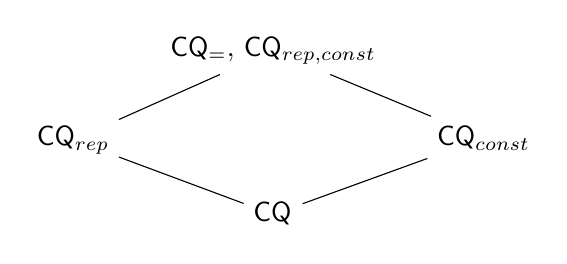
\begin{tikzpicture}
		\node (t)                          {\cq{=}, \cq{rep,const}};
		\node (l) [below left =0.75cm of t] {\cq{rep}};
		\node (r) [below right=0.75cm of t] {\cq{const}};
		\node (b) [below      =1.50cm of t] {\cq{}};
		\draw (b) -> (l);
		\draw (b) -> (r);
		\draw (l) -> (t);
		\draw (r) -> (t);
\end{tikzpicture}
\end{center}

\end{multicols}

\bibliography{2}

\end{document}